Prior to proposal presentation, we created system block diagrams for how the various systems are to function within the system.

\begin{figure}[htbp]
    \centering
    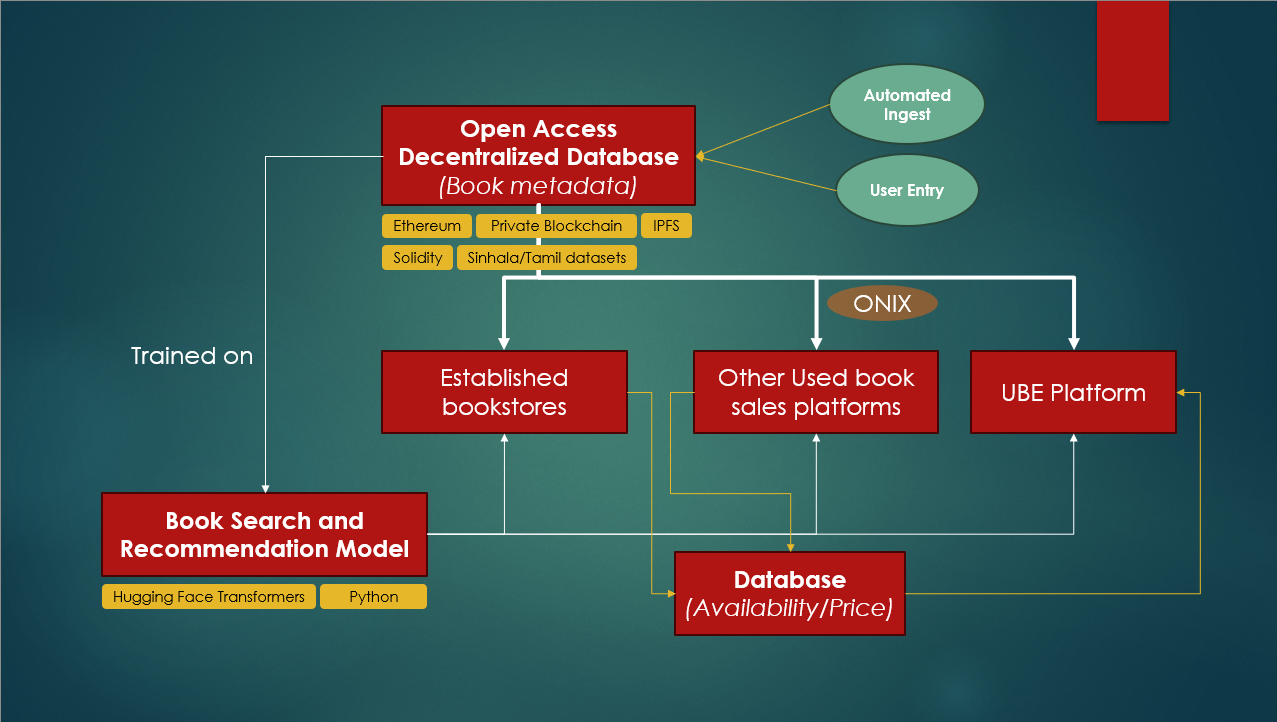
\includegraphics[width=1\textwidth]{../../assets/proposal_block_diagram.png}
    \caption{Block Diagram for Proposed System}
    \label{fig:example}
\end{figure}

As per our proposal, we identified 4 key deliverables necessary to succeed in our project, namely:

\begin{itemize}
    \item Book Data Database
    \item Recommendation System APIs
    \item Search APIs
    \item Demo applications
\end{itemize}

Initially we began our project with data collection, analysis, and planning. We obtained book metadata from various sources, chiefly,
\begin{itemize}
    \item Libgen.rs database dumps
    \item malcolmosh's excellend goodbooks-10k-extended dataset
    \item Sri Lanka National Library's Sri Lanka National Bibliography
\end{itemize}

The first two sources were preformatted and easy to use data, which was used to train our base recommender model, which functions in English language. We were unable to fully exploit the SLNB data, as data extraction proved to be beyond our current capacity.

Utilizing the pdfplumber package in Python, we were able to extract tokens for every word in the bibliography. (see Appendix \ref{appendix-b} for a sample of the extracted data.)

Utilizing the fitz package, we were able to extract a more structured representation of the data. The issues faced when analyzing this data will be explained in detail in the discussion section.

\begin{figure}[htbp]
    \centering
    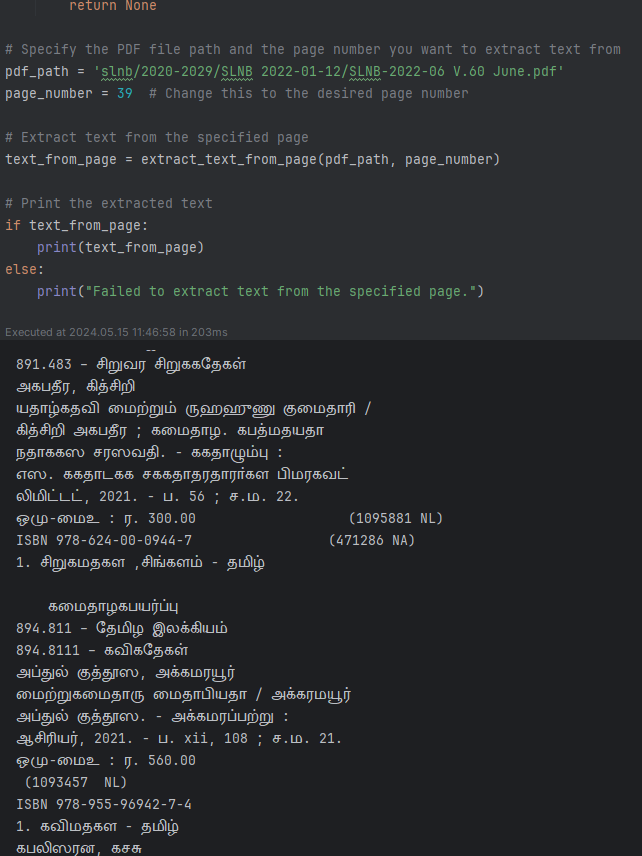
\includegraphics[width=1\textwidth]{../../assets/extracted.png}
    \caption{Data extracted using fitz}
    \label{fig:extracted}
\end{figure}

\newpage

Next, we began architecting the applications necessary to implement the system. We decided to use Git for version control. Though there were other options such as mercurial available, the widespread use of Git and familiarity with it prompted us to choose it as our VCS software of choice.